%% ------------------------------------------------------------------------- %%
\chapter{Modelagem}
\label{cap:modelagem}

Utilizando-se da base de dados para modelagem descrita na Seção "Criação da base para modelagem" (\ref{sec:criacao_da_base_para_modelagem}) - cujas variáveis explicativas foram descritas na Seção "Variáveis Explicativas" (\ref{sec:variaveis_explicativas}) e a variável resposta descrita na Seção "Variável Resposta" (\ref{sec:variavel_resposta}) - foram aplicados modelos de aprendizado de máquina com o intuito de obter o melhor desempenho para predição da variável resposta utilizando as variáveis explicativas construídas.

Os métodos de aprendizado de máquina utilizados foram Regressão Linear, Random Forest e XGBoost, sendo que a afinação dos parâmetros de tais modelos foi feita utilizando-se o método Randomized Search. A avaliação de desempenho destes modelos foi feita utilizando-se de duas métricas, a raiz do erro quadrático médio e as bandas de acerto, e a interpretação dos modelos Random Forest e XGBoost foram feitas por meio do método Shapley Value.

\section{Análise Descritiva}
\label{sec:analise_descritiva}

A análise descritiva consiste em explorar dados utilizados para a modelagem com o intuito de encontrar a existência, ou não, de uma relação causal entre as variáveis explicativas e a variável resposta. Neste trabalho já foram apresentadas algumas análises descritivas no Capítulo \ref{cap:contexto}, como, por exemplo, as estatísticas dos percentuais de polaridade obtidos da variável resposta.

Foram utilizadas 52 variáveis explicativas neste trabalho, foi realizado uma análise em cada uma das variáveis utilizando-se de gráficos de dispersão com a variável resposta. Nestes gráficos de dispersão, os valores observados para a variável explicativa estão dispostos no eixo das ordenadas e os valores observados para a variável resposta estão dispostos no eixo das abscissas. Como exemplo, o gráfico de dispersão - que se encontra no anexo \ref{ape:cap3_scatter_plot} - da variável \verb|'family_var_01_inappropriate_pct'| (que se trata do percentual de domicílios particulares permanentes em situação inadequada por município em 2000 dividido pela mesma informação em 2010), nota-se uma relação linear positiva média entre a variável explicativa e a variável resposta. Os gráficos de dispersão de todas as variáveis explicativas se encontram no anexo \ref{ape:cap3_scatter_plot}.

O código citado no parágrafo anterior foi escrito na linguagem de programação Python utilizando a ferramenta Notebook Jupyter e se encontra no anexo \ref{ape:model_visualization}.

\section{Randomized Search}
\label{sec:randomized_search}

O Randomized Search é um método utilizado para otimização de hiperparâmetros que consiste em uma pesquisa aleatória sobre os hiperparâmetros fornecidos para treinamento de modelos de aprendizado de máquina visando o melhor desempenho de tal modelo. Neste trabalho foi escolhido utilizar-se o Randomized Search frente aos dois métodos mais utilizados na atualidade - o Grid Search (uma pesquisa exaustiva por meio de um subconjunto especificado manualmente do espaço de hiperparâmetros de um algoritmo de aprendizado) e a busca manual - uma vez que o Randomized Search realiza buscas mais eficientes que o Grid Search e a busca manual (ver \citet{Bergstra2012}).

Foi-se utilizada a implementação deste método proveniente da biblioteca em Python Scikit-learn (\citet{Sklearn}). Ao contrário do Grid Search, nem todos os valores dos parâmetros são testados, mas um número fixo de configurações de parâmetros é amostrado das distribuições especificadas. O número de configurações de parâmetros que são tentadas é definido pela quantidade de iterações passadas ao método e o desempenho do modelo de aprendizado de máquina treinado após a escolha dos hiperparâmetros é calculado utilizando-se do método de validação cruzada.

Se todos os parâmetros forem apresentados como uma lista, é realizada a amostragem sem reposição. Se pelo menos um parâmetro for fornecido como distribuição, é utilizada a amostragem com reposição. No âmbito deste trabalho, alguns parâmetros foram fornecidos como lista e outros como distribuição, assim, para o treinamento do modelo de aprendizado de máquina Random Forest foi-se utilizado uma amostragem com reposição e para o treinamento do modelo de aprendizado de máquina XGBoost foi-se utilizado uma amostragem sem reposição.

Além do Randomized Search ser a melhor opção por sua eficiência, existe a motivação da viabilidade da otimização dos hiperparâmetros, uma vez que para o treinamento do modelo de aprendizado de máquina XGBoost foi-se utilizado dez diferentes hiperparâmetros com diferentes quantidades de valores, representando no final uma quantidade de 1.411.200 possibilidades de cenários distintos para o treinamento.

\section{Shapley Value}
\label{sec:shapley_value}

O Shapley Value é uma proposta de solução na teoria dos jogos cooperativos, foi nomeado em homenagem a Lloyd Shapley que o definiu inicialmente (ver \citet{Shapley1953}).

Em um cenário de jogos cooperativos onde, para cada jogo cooperativo, atribui-se uma distribuição única (entre os jogadores) de um excedente total gerado pelo grupo de todos os jogadores, o Shapley Value é caracterizado como uma coleção de propriedades para explicação da proveniência de cada parte desse excedente total.

A configuração é da seguinte forma: um grupo de jogadores coopera e obtém um certo ganho geral com essa cooperação. Como alguns jogadores podem contribuir mais para o grupo do que outros, ou podem ter um poder de barganha diferente, qual a importância de cada jogador para a cooperação geral e que recompensa ele pode razoavelmente esperar? Esta pergunta é uma das motivações para criação do Shapley Value, i.e., explicar essa importância individual e a recompensa esperada.

O paralelo da explicação acima à explicação do algoritmo em aprendizado de máquina seria de que os jogadores são as variáveis explicativas, o ganho geral obtido por cada jogador é o impacto na predição do modelo e a importância individual seria a importância da variável explicativa no modelo. A importância das variáveis explicativas em modelos de aprendizado de máquina é uma informação amplamente discutida, uma vez que existem diferentes formas de se calcular tal importância e, muitas vezes, a ordenação da importância das variáveis pode ser diferente de um método para outro gerando discussão sobre a escolha do melhor método a ser utilizado.

O Shapley Value vem sendo considerado a forma mais robusta e consistente de se avaliar a importância das variáveis explicativas em um modelo (ver \citet{Lundberg2017}), ele será utilizado neste trabalho tanto para ordenação da importância das variáveis quanto para interpretação das variáveis explicativas utilizadas no modelo. Foi-se utilizada a implementação deste método proveniente da biblioteca em Python SHAP (\citet{Shap}).

Uma simplificação de como o Shapley Value pode ser calculado para uma determinada variável explicativa $j$ pode ser dada pela fórmula abaixo (considere f o modelo que se deseja avaliar o impacto das variáveis explicativas).

\begin{equation}
\hat{\phi}_j = \frac{1}{M} \sum^{M}_{m=1}(\hat{f}(x^m_{+j}) - \hat{f}(x^m_{-j}))
\end{equation}

Onde,

\begin{itemize}
	\item $ \hat{f}(x^m_{+j}) $ é a predição para $ x^m_{+j} $, sendo que $ x^m_{+j} $ é um vetor de variáveis explicativas provindas de uma observação aleatória z (z é uma observação aleatória selecionada da base de treinamento), exceto pelo valor da variável explicativa que corresponde à j.
	\item o vetor $ x^m_{-j} $ é quase idêntico ao vetor $ x^m_{+j} $ com a diferença de que o valor $ x^m_j $ é tomado da observação aleatória z.
\end{itemize}

Assim, o algoritmo para se calcular o Shapley Value é dado por:

\begin{itemize}
	\item Para $ m=1,...,M $, onde M é o total de iterações e p é o total de variáveis explicativas:
	\begin{itemize}
		\item Selecione duas observações aleatórias (vetores x e z) de todas observações disponíveis na base de treinamento
		\item Selecione uma permutação aleatória das variáveis explicativas
		\item Obtenha o vetor $ x_0 = (x_{(1)},...,x_{(j)},...,x_{(p)}) $
		\item Obtenha o vetor $ z_0 = (z_{(1)},...,z_{(j)},...,z_{(p)}) $
		\item Construa dois vetores:
		\begin{itemize}
			\item Com a variável j: $ x_{+j} = (x_{(1)},...,x_{(j-1)},x_{(j)},z_{(j+1)},...,z_{(p)}) $
			\item Sem a variável j: $ x_{-j} = (x_{(1)},...,x_{(j-1)},z_{(j)},z_{(j+1)},...,z_{(p)}) $
		\end{itemize}
		\item Calcule a contribuição marginal: $ \phi_j^m = \hat{f}(x^m_{+j}) - \hat{f}(x^m_{-j}) $
	\end{itemize}
	\item Calcule o Shapley Value como a média: $ \hat{\phi}_j = \frac{1}{M} \sum^{M}_{m=1}(\phi_j^m) $
\end{itemize}

\section{Métricas para avaliação de desempenho}
\label{sec:metricas_avaliacao}

Neste trabalho serão utilizadas duas métricas para avaliação de desempenho, a raiz do erro quadrático médio e a banda de acerto.

A raiz do erro quadrático médio (do inglês root mean squared error, RMSE) é uma medida frequentemente usada das diferenças entre os valores previstos por um modelo ou estimador e os valores observados. O RMSE representa a raiz quadrada da média quadrática das diferenças entre os valores previstos e os valores observados. Esses desvios são chamados de resíduos, quando os cálculos são realizados sobre a amostra de dados usada para estimativa, ou são chamados de erros (ou erros de previsão), quando calculados fora da amostra. O RMSE é uma medida de precisão, para comparar erros de previsão de diferentes modelos para um conjunto de dados específico e não entre conjuntos de dados, pois depende da escala.

O RMSE é sempre não negativo e um valor 0 (quase nunca alcançado na prática) indicaria um ajuste perfeito para os dados. Em geral, um RMSE mais baixo é melhor que um mais alto. No entanto, comparações entre diferentes tipos de dados seriam inválidas porque a medida depende da escala dos números usados. Neste trabalho, as medidas de RMSE são comparáveis uma vez que os dados trabalhados são os mesmos mudando apenas os modelos.

\begin{equation}
\mathbf {RMSE} ={\sqrt {\frac {\sum _{t=1}^{N}({\hat {y}}_{t}-y_{t})^{2}}{N}}}
\end{equation}

Sendo que,

\begin{itemize}
    \item $ \hat y_t $ representa o valor predito do modelo
    \item $ y_t $ representa o valor observado
    \item $ N $ representa a quantidade de observações
\end{itemize}

A banda de acerto é uma medida para avaliar a distribuição dos erros de predição separando-os em três categorias interpretáveis. De acordo com o valor de predição do modelo, se classifica tal predição em cada banda, tais bandas são catalogadas como "subestimado", "bem estimado" e "superestimado". As regras para classificação em cada uma dessas opções estão listadas abaixo. O valor de $ \delta $ foi determinado empiricamente após sucessivos testes como sendo 0.05.

\begin{itemize}
	\item Subestimado: Se o valor da predição for menor que o valor observado menos $ \delta $
	\item Superestimado: Se o valor da predição for maior que o valor observado mais $ \delta $
	\item Bem estimado: Se o valor da predição estiver entre o valor observado menos $ \delta $ e o valor observado mais $ \delta $
\end{itemize}

\section{Regressão Linear}
\label{sec:regressao_linear}

A regressão linear é uma abordagem para modelar a relação entre uma variável resposta (ou variável dependente) contínua e uma ou mais variáveis ​​explicativas (ou variáveis ​​independentes). É chamado de regressão linear simples quando se usa apenas uma variável explicativa, e regressão linear múltipla quando se usa mais de uma variável explicativa. Neste trabalho utilizaremos a regressão linear múltipla.

Os relacionamentos são modelados usando funções preditivas lineares cujos parâmetros desconhecidos do modelo são estimados a partir dos dados. Mais comumente, assume-se que a média condicional da resposta, dados os valores das variáveis ​​explicativas (ou preditores), seja uma função afim desses valores (função afim também é conhecida como transformação linear ($ Ax $) seguida por uma translação ($ +b $)). Como todas as formas de análise de regressão, a regressão linear se concentra na distribuição de probabilidade condicional da resposta, dados os valores dos preditores, e não na distribuição de probabilidade conjunta de todas essas variáveis.

A regressão linear foi o primeiro tipo de análise de regressão a ser estudada rigorosamente e usada extensivamente em aplicações práticas. Isso ocorre porque os modelos que dependem linearmente de seus parâmetros desconhecidos são mais fáceis de ajustar do que os modelos não linearmente relacionados aos seus parâmetros, e porque as propriedades estatísticas dos estimadores resultantes são mais fáceis de se determinar.

A regressão linear tem muitos usos práticos, o utilizado neste trabalho é o de previsão. A regressão linear pode ser usada para ajustar um modelo preditivo a um conjunto de dados observado de valores da resposta e variáveis ​​explicativas. Depois de desenvolver esse modelo, se valores adicionais das variáveis ​​explicativas forem coletados sem um valor de resposta definido, o modelo ajustado pode ser usado para fazer uma previsão da resposta.

Os modelos de regressão linear geralmente são ajustados usando a abordagem de mínimos quadrados, mas também podem ser ajustados de outras maneiras como minimizando uma versão penalizada da função custo de mínimos quadrados como na regressão de Ridge (penalidade de norma L2) e LASSO (penalidade de norma L1), mais informações de como funcionam tais técnicas de penalidade ver \citet{SantosaAndSymes1986} e \citet{Tibshirani1996}.

Dado um conjunto de dados $ {\displaystyle \{y_{i},\,x_{i1},\ldots ,x_{ip}\}_{i=1}^{n}} $ de dimensão n, um modelo de regressão linear pressupõe que a relação entre a variável dependente $ y $ e o vetor de regressores $ x $ é linear. Essa relação é modelada através de uma variável de erro $ \varepsilon $ - uma variável aleatória não observada que adiciona "ruído" à relação linear entre a variável dependente e os regressores. Assim, o modelo assume a forma:

\begin{equation}
{\displaystyle y_{i}=\beta _{0}+\beta _{1}x_{i1}+\cdots +\beta _{p}x_{ip}+\varepsilon _{i}=\mathbf {x} _{i}^{\mathsf {T}}{\boldsymbol {\beta }}+\varepsilon _{i},\qquad i=1,\ldots ,n,}
\end{equation}

onde T denota a transposição, de modo que $ {x}_{i}^{\mathsf {T}}{\boldsymbol {\beta }} $ é o produto interno entre os vetores $ {x}_{i} $ e $ \beta $.

Essas equações também podem ser representadas na notação matricial, como

\begin{equation}
{\displaystyle \mathbf {y} =X{\boldsymbol {\beta }}+{\boldsymbol {\varepsilon }},\,}
\end{equation}

onde

\mathbf {y} ={\begin{pmatrix}y_{1}\\y_{2}\\\vdots \\y_{n}\end{pmatrix}}, X={\begin{pmatrix}\mathbf {x} _{1}^{\mathsf {T}}\\\mathbf {x} _{2}^{\mathsf {T}}\\\vdots \\\mathbf {x} _{n}^{\mathsf {T}}\end{pmatrix}}={\begin{pmatrix}1&x_{11}&\cdots &x_{1p}\\1&x_{21}&\cdots &x_{2p}\\\vdots &\vdots &\ddots &\vdots \\1&x_{n1}&\cdots &x_{np}\end{pmatrix}}, {\boldsymbol {\beta }}={\begin{pmatrix}\beta _{0}\\\beta _{1}\\\beta _{2}\\\vdots \\\beta _{p}\end{pmatrix}, {\boldsymbol {\varepsilon }}={\begin{pmatrix}\varepsilon _{1}\\\varepsilon _{2}\\\vdots \\\varepsilon _{n}\end{pmatrix}}.}

Sendo que,

\begin{itemize}
	\item $ \mathbf {y} $ é um vetor de valores observados $ y_{i} (i = 1, \ldots, n) $ também conhecido como variável resposta ou variável dependente. Essa variável não deve ser confundida com os valores previstos, que são indicados como $ \hat{y} $. A decisão sobre qual variável em um conjunto de dados ser modelada como variável dependente e quais são modeladas como variáveis ​​independentes baseia-se na presunção de que o valor de uma das variáveis ​​é causado por, ou diretamente influenciado por outras variáveis.

	\item $ X $ pode ser visto como uma matriz de vetores de linha $ \mathbf {x}_{i} $, conhecidos como variáveis ​​explicativas ou variáveis ​​independentes. Geralmente, uma constante é incluída como um dos regressores, o elemento correspondente de $ \beta $ é chamado de intercepto. Muitos procedimentos de inferência estatística para modelos lineares exigem a presença de um intercepto, por isso o mesmo é frequentemente incluído mesmo que considerações teóricas sugiram que seu valor seja zero.

	\item $ \beta $ é um vetor de parâmetro dimensional $ (p + 1) $, em que $ \beta_{0} $ é o termo de intercepto, se houver um no modelo - caso contrário, $ \beta $ é p-dimensional. Seus elementos são conhecidos como efeitos ou coeficientes de regressão, embora o último termo as vezes seja reservado para os efeitos estimados. A estimativa estatística e inferência na regressão linear se concentra em $ \beta $, os elementos desse vetor de parâmetro são interpretados como derivadas parciais da variável dependente em relação às várias variáveis ​​independentes.

	\item $ \varepsilon $ é um vetor de valores $ \varepsilon_{i} $. Essa parte do modelo é chamada de termo de erro ou, as vezes, ruído. Essa variável captura todos os outros fatores que influenciam a variável dependente $ y $, exceto os regressores $ x $. A relação entre o termo de erro e os regressores, por exemplo, sua correlação, é uma consideração crucial na formulação de um modelo de regressão linear, pois determinará o método de estimativa apropriado.
\end{itemize}

Uma explicação mais detalhada sobre como a regressão linear estima seus parâmetros pode ser encontrada em \citet{Freedman2009}.

Neste trabalho, o treinamento da regressão linear foi feito utilizando-se a biblioteca em Python scikit-learn (\citet{Sklearn}) que é uma das bibliotecas mais utilizadas para treinamento de modelos de aprendizado de máquina na linguagem de programação Python.

\section{Resultados da Regressão Linear}
\label{sec:resultados_regressao_linear}

O modelo de regressão linear é relativamente simples e de fácil interpretabilidade, uma boa estratégia de modelagem é no início do processo de modelagem realizar o treinamento do mesmo e utilizar seu desempenho como base para comparação futura com outros experimentos utilizando-se de outros modelos de aprendizado de máquina. Assim, tal modelo foi utilizado apenas para obter um desempenho base.

As estimativas para os parâmetros deste modelo estão dispostas na tabela abaixo.

\begin{table}[h]
\centering
\caption{Estimativas da regressão linear}
\label{tab:cap3_estimativa_reg_lin}
\begin{adjustbox}{width=\textwidth}
\begin{tabular}{cc}
Variável ou Categoria & Estimativa \\
\hline
\verb|education_var_01_quantity_pct| &  0.06117 \\
\verb|family_var_01_suitable_pct|  & -0.00021 \\
\verb|family_var_01_semi_suitable_pct| &  0.00140 \\
\verb|family_var_01_inappropriate_pct|  & -0.00055 \\
\verb|fertility_var_01_has_children_pct| &  0.02855 \\
\verb|fertility_var_01_children_born_pct| &  0.25068 \\
\verb|fertility_var_01_children_borned_live_pct|  & -0.28298 \\
\verb|fertility_var_01_children_borned_dead_pct|  & -0.00617 \\
\verb|fertility_var_02_married_pct| &  0.03087 \\
\verb|fertility_var_02_separated_pct|  & -0.00328 \\
\verb|fertility_var_02_divorced_pct| &  0.00997 \\
\verb|fertility_var_02_widow_pct| &  0.01008 \\
\verb|fertility_var_02_single_pct| &  0.06214 \\
\verb|fertility_var_03_total_pct| &  0.16219 \\
\verb|work_var_01_regular_pct| &  0.03426 \\
\verb|work_var_01_irregular_pct| &  0.04609 \\
\verb|social_indicator_var_01_15_to_24_years_pct|  & -0.00144 \\
\verb|social_indicator_var_01_25_to_59_years_pct|  & -0.02038 \\
\verb|social_indicator_var_01_60_to_more_years_pct| &  0.00484 \\
\verb|social_indicator_var_02_suitable_pct|  & -0.00088 \\
\verb|social_indicator_var_02_semi_suitable_pct|  & -0.01605 \\
\verb|social_indicator_var_02_inappropriate_pct|  & -0.00055 \\
\verb|social_indicator_var_03_responsable_illiterate_pct| &  0.01571 \\
\verb|social_indicator_var_03_inappropriate_residence_pct|  & -0.00011 \\
\verb|social_indicator_var_03_responsable_illiterate_and_inappropriate_residence_pct| &  0.00063 \\
\verb|enem_var_01_enem_score_mean_pct| &  0.33489 \\
\verb|enem_var_01_enem_score_std_pct|  & -0.01912 \\
\verb|enem_var_01_enem_score_median_pct|  & -0.34682 \\
\verb|state_ac|  & -0.07552 \\
\verb|state_al| &  0.01843 \\
\verb|state_ba| &  0.01230 \\
\verb|state_ce|  & -0.00753 \\
\verb|state_es| &  0.01247 \\
\verb|state_go| &  0.03169 \\
\verb|state_ma| &  0.06556 \\
\verb|state_mg| &  0.04068 \\
\verb|state_ms|  & -0.00889 \\
\verb|state_mt| &  0.00559 \\
\verb|state_pa| &  0.00188 \\
\verb|state_pb| &  0.02969 \\
\verb|state_pe| &  0.00794 \\
\verb|state_pi|  & -0.00892 \\
\verb|state_pr|  & -0.00117 \\
\verb|state_rj|  & -0.00751 \\
\verb|state_rn| &  0.00427 \\
\verb|state_ro| &  0.01943 \\
\verb|state_rr|  & -0.02139 \\
\verb|state_rs|  & -0.02576 \\
\verb|state_sc|  & -0.01996 \\
\verb|state_se| &  0.01385 \\
\verb|state_sp|  & -0.02229 \\
\verb|state_to|  & -0.06484 \\
\hline
\end{tabular}
\end{adjustbox}
\end{table}
\FloatBarrier

Nota-se que em alguns casos houve inversão de estimativas com relação ao esperado, como exemplo de tal inversão temos os gráficos de dispersão da variáveis explicativas \verb|"enem_var_01_enem_score_mean_pct"| e \verb|"enem_var_01_enem_score_media| \\ \verb|n_pct"| (presentes no apêndice \ref{ape:cap3_scatter_plot}). Tais gráficos mostram uma dispersão de valores muito próxima entre as duas variáveis, conceitualmente também é esperado que a relação com a variável resposta seja semelhante, porém as estimativas são estritamente opostas assumindo os valores 0.33489 e -0.34682, respectivamente.

O desempenho do modelo foi avaliado, conforme mencionado anteriormente, utilizando-se as medidas RMSE e bandas de acerto. Na tabela abaixo apresenta-se o RMSE sobre a base de treinamento ("Treino"), sobre a base de validação ("Validação"), sobre a base de validação utilizando-se um modelo aleatório ("Validação (modelo aleatório)") e sobre a base de validação utilizando-se um modelo nulo ("Validação (modelo nulo)"). O modelo aleatório apresenta um número aleatório que esteja entre o mínimo e o máximo observado na validação, foi criado apenas para critério de comparação com o modelo de regressão linear, assim como o modelo nulo, sendo que o modelo nulo é a média da variável resposta na base de treinamento. Nota-se um erro estritamente superior do modelo aleatório sobre o erro da regressão linear, o que implica que o modelo teve assertividade em suas predições e também que existe a possibilidade de previsão da variável resposta utilizando-se as variáveis explicativas criadas neste trabalho.

\begin{table}[h]
\centering
\caption{RMSE resultante da regressão linear}
\label{tab:cap3_rmse_reg_lin}
\begin{tabular}{cc}
Base & Estatística \\
\hline
Treino & 0.0484 \\
Validação & 0.0628 \\
Validação (modelo aleatório) & 0.1868 \\
Validação (modelo nulo) & 0.0525 \\
\hline
\end{tabular}
\end{table}
\FloatBarrier

Na tabela abaixo apresenta-se a banda de acerto sobre a base de treinamento ("Treino"), sobre a base de validação ("Validação"), sobre a base de validação utilizando-se um modelo aleatório ("Validação (modelo aleatório)") e sobre a base de validação utilizando-se um modelo nulo ("Validação (modelo nulo)"). Nota-se que a regressão linear teve a maior concentração em "Bem Estimado" com 65\% na validação, e 75\% no treino.

\begin{table}[h]
\centering
\caption{Banda de acerto da regressão linear}
\label{tab:cap3_band_reg_lin}
\begin{tabular}{cccc}
Base & Subestimado & Bem Estimado & Superestimado \\
\hline
Treino & 0.1262 & 0.75 & 0.1238 \\
Validação & 0.1786 & 0.65 & 0.1714 \\
Validação (modelo aleatório) & 0.3929 & 0.2928 & 0.3143 \\
Validação (modelo nulo) & 0.1214 & 0.7143 & 0.1643 \\
\hline
\end{tabular}
\end{table}
\FloatBarrier

No gráfico abaixo nota-se, apesar de suave, uma relação de linearidade entre os valores preditos (eixo das ordenadas) e os valores observados (eixo das abscissas) em ambas bases de dados (treino e validação).

\graphicspath{ {./figuras/model_performance/} }
\begin{center}
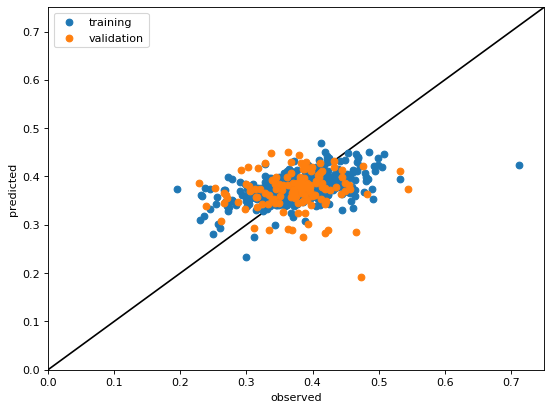
\includegraphics[width=12.0cm, keepaspectratio]{cap3_scatter_reg_lin}
\captionof{figure}{Gráfico de dispersão da Regressão Linear}
\label{ape:cap3_scatter_reg_lin}
\end{center}

\section{Random Forest}
\label{sec:random_forest}

O Random Forest é um método de aprendizado de máquina para classificação e regressão que opera construindo várias árvores de decisão (para classificação) ou árvores de regressão (para regressão), sendo que a predição de tal método é dada pela moda dos valores preditos em cada árvore, no caso da classificação, ou é dada pela média dos valores preditos em cada árvore, no caso de regressão. A forma de seleção aleatória das árvores reduz a incidência de overfitting no treino sobre a base de treinamento.

O Random Forest foi criado por Tin Kam Ho em \citet{Ho1995} usando o método do subespaço aleatório, que, na formulação de Ho, é uma maneira de implementar a abordagem de "discriminação estocástica" à classificação proposta por Eugene Kleinberg (ver \citet{Kleinberg1990}).

O algoritmo é primordialmente baseado em árvores de decisão que é um método popular para várias tarefas de aprendizado de máquina. A árvore de decisão atende aos requisitos para servir como um procedimento de prateleira para mineração de dados, porque é invariável à escala e transformações em variáveis explicativas, é robusto para inclusão de variáveis irrelevantes e seu resultado, na maioria das vezes, é interpretável.

Em particular, árvores muito profundas tendem a aprender padrões altamente irregulares: elas superestimam seus conjuntos de treinamento, ou seja, têm um viés baixo, mas uma variância muito alta (comumente conhecido como bias-variance tradeoff). O Random Forest é uma maneira de calcular a média de várias árvores de decisão, treinadas em diferentes partes do mesmo conjunto de treinamento, com o objetivo de reduzir a variância. Isso ocorre às custas de um pequeno aumento no viés e perda de interpretabilidade - uma vez que são criadas diversas árvores -, mas geralmente se aumenta muito o desempenho no modelo final.

O algoritmo de treinamento para o Random Forest aplica a técnica geral de agregação de bootstrap conhecida como Bagging. Dado um conjunto de treinamento $ {\displaystyle X = x_{1},\ldots ,x_{n}} $ com respostas $ {\displaystyle Y = y_{1},\ldots ,y_{n}} $, selecionados repetidamente $ B $ vezes, seleciona-se uma amostra aleatória com repetição do conjunto de treinamento e se realiza o treinamento das árvores a essas amostras:

Para $ b = 1, ..., B $ :

\begin{enumerate}
	\item Amostra, com repetição, $ n $ exemplos de treinamento de $ X, Y $, chamados de $ X_b, Y_b $.
	\item Treine uma árvore de classificação ou regressão $ f_b $ em $ X_b, Y_b $.
\end{enumerate}

Após o treinamento, predições para amostras não vistas $ x' $ podem ser feitas calculando a média das predições de todas as árvores de regressão individuais em $ x' $:

\begin{equation}
{\displaystyle {\hat {f}}={\frac {1}{B}}\sum _{b=1}^{B}f_{b}(x')}
\end{equation}

Ou, no caso de árvores de classificação, utilizando-se o voto da maioria.

O procedimento de bootstrapping leva a um melhor desempenho do modelo pois diminui a variância do modelo, sem aumentar o viés. Isso significa que, embora as previsões de uma única árvore sejam altamente sensíveis ao ruído em seu conjunto de treinamento, a média de muitas árvores não é, desde que as árvores não estejam correlacionadas. Simplesmente treinar muitas árvores em um único conjunto de treinamento daria árvores altamente correlacionadas (ou até a mesma árvore muitas vezes, se o algoritmo de treinamento for determinístico). A amostragem por bootstrapping é uma maneira de descorrelacionar as árvores, utilizando-se diferentes conjuntos de treinamento.

O procedimento descrito acima trata do algoritmo original de bagging para árvores. O Random Forest difere apenas por uma característica específica, ele utiliza um algoritmo de aprendizado de árvore modificado que seleciona, a cada divisão do aprendizado da árvore, um subconjunto aleatório de variáveis explicativas. A motivação para tal vem da correlação das árvores em uma amostra de bootstrap comum, i.e., se uma ou algumas variáveis explicativas são preditores muito fortes para a variável de resposta, esses recursos serão selecionados em muitas das árvores B causando uma alta correlação entre as árvores treinadas.

Geralmente utiliza-se, para um problema de classificação com $ p $ variáveis explicativas, $ \sqrt{p} $ (arredondado para baixo) variáveis explicativas ​​em cada divisão. Para problemas de regressão, recomenda-se $ p/3 $ (arredondado para baixo). Contudo, na prática, os melhores valores para esses parâmetros dependerão do problema e devem ser tratados na otimização dos hiperparâmetros.

Neste trabalho, o treinamento do random forest foi feito utilizando-se a biblioteca em Python scikit-learn (\citet{Sklearn}) na linguagem de programação Python.

\section{Resultados do Random Forest}
\label{sec:resultados_random_forest}

O treinamento do modelo Random Forest utilizou-se da metodologia explicada na Seção \ref{sec:randomized_search} e os hiperparâmetros testados foram:

\begin{itemize}
	\item \verb|max_depth|: Profundidade máxima da árvore.
	\item \verb|max_features|: Número de variáveis explicativas a serem consideradas ao procurar a melhor divisão da árvore.
	\item \verb|min_samples_split|: Número mínimo de amostras necessárias para se dividir um nó da árvore.
	\item \verb|min_samples_leaf|: Número mínimo de amostras necessárias para se deixar em uma folha da árvore.
	\item \verb|n_estimators|: Número de árvores na floresta.
	\item \verb|bootstrap|: Se amostras de bootstrap são usadas na construção das árvores.
	\item \verb|criterion|: Função a ser usada para medir a qualidade da divisão da árvore (erro quadrático médio, erro absoluto médio, etc.).
\end{itemize}

O número de iterações no Randomized Search a serem realizadas foi de 300 com um método de validação cruzada 5-fold (\citet{Kohavi1995}). Por fim, o modelo final após a otimização do Randomized Search possui os hiperparâmetros apresentados na tabela abaixo.

\begin{table}[h]
\centering
\caption{Hiperparâmetros finais do Random Forest}
\label{tab:cap3_parametros_random_forest}
\begin{tabular}{cc}
Hiperparâmetro & Valor \\
\hline
\verb|max_depth| & 10 \\
\verb|max_features| & 13 \\
\verb|min_samples_split| & 0.4774005510811298 \\
\verb|min_samples_leaf| & 0.05170415106602393 \\
\verb|n_estimators| & 75 \\
\verb|bootstrap| & False \\
\verb|criterion| & mse \\
\hline
\end{tabular}
\end{table}
\FloatBarrier

O modelo Random Forest não é de fácil interpretabilidade, apesar de ser possível ver e analisar a estrutura de cada uma das árvores separadamente que compõem o mesmo, não é direta a interpretação de como foi feita a predição dos valores por tal algoritmo. Assim, para interpretar como cada variável afeta o modelo e avaliar a importância de cada uma delas utilizamos o método de Shapley Values (descrito na Seção \ref{sec:shapley_value}), sendo que o gráfico resultante se encontra abaixo.

\graphicspath{ {./figuras/model_performance/} }
\begin{center}
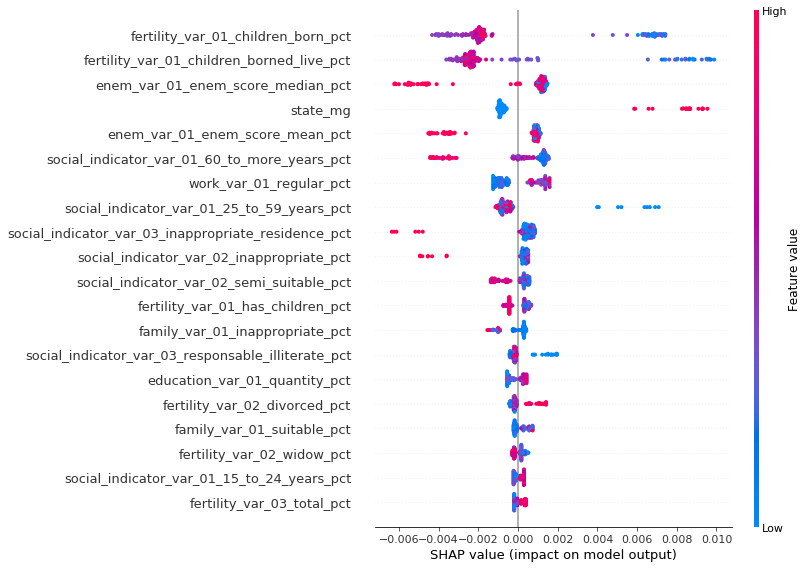
\includegraphics[width=14.0cm, keepaspectratio]{cap3_shap_random_forest}
\captionof{figure}{Shapley value do Random Forest}
\label{ape:cap3_shap_random_forest}
\end{center}

No gráfico, as variáveis apresentadas à esquerda estão ordenadas de forma decrescente em nível de importância no modelo, no eixo das ordenadas se apresentam os valores de Shapley Values - que pode ser lido como a influência no valor de predição do modelo, tanto positivo quanto negativo -, e as cores como o valor da variável explicativa propriamente dita, sendo vermelho o maior valor possível e azul o menor valor possível para a variável em questão. Então, no caso da variável \verb|fertility_var_01_children_born_pct| - que se trata do percentual de crianças nascidas por município em 2000 dividido pela mesma informação em 2010 -, a interpretação se dá na forma de que quanto menor o valor de tal variável, mais positiva será a influência sobre a predição de polaridade negativa no relatório do município em questão.

Assim como a regressão linear, o desempenho do modelo foi avaliado utilizando-se as medidas RMSE e bandas de acerto. Na tabela abaixo apresenta-se o RMSE sobre a base de treinamento ("Treino"), sobre a base de validação ("Validação"), sobre a base de validação utilizando-se um modelo aleatório ("Validação (modelo aleatório)") e sobre a base de validação utilizando-se um modelo nulo ("Validação (modelo nulo)"). O modelo aleatório apresenta um número aleatório que esteja entre o mínimo e o máximo observado na validação, foi criado apenas para critério de comparação com o modelo Random Forest, assim como o modelo nulo, sendo que o modelo nulo é a média da variável resposta na base de treinamento. Nota-se um erro estritamente superior do modelo aleatório sobre o erro do Random Forest.

\begin{table}[h]
\centering
\caption{RMSE resultante do Random Forest}
\label{tab:cap3_rmse_random_forest}
\begin{tabular}{cc}
Base & Estatística \\
\hline
Treino & 0.0513 \\
Validação & 0.0527 \\
Validação (modelo aleatório) & 0.1728 \\
Validação (modelo nulo) & 0.0525 \\
\hline
\end{tabular}
\end{table}
\FloatBarrier

Na tabela abaixo apresenta-se a banda de acerto sobre a base de treinamento ("Treino"), sobre a base de validação ("Validação"), sobre a base de validação utilizando-se um modelo aleatório ("Validação (modelo aleatório)") e sobre a base de validação utilizando-se um modelo nulo ("Validação (modelo nulo)"). Nota-se que o Random Forest teve a maior concentração em "Bem Estimado" com mais de 70\% na validação e treino.

\begin{table}[h]
\centering
\caption{Banda de acerto do Random Forest}
\label{tab:cap3_band_random_forest}
\begin{tabular}{cccc}
Base & Subestimado & Bem Estimado & Superestimado \\
\hline
Treino & 0.1333 & 0.731 & 0.1357 \\
Validação & 0.1357 & 0.7286 & 0.1357 \\
Validação (modelo aleatório) & 0.5214 & 0.1215 & 0.3571 \\
Validação (modelo nulo) & 0.1214 & 0.7143 & 0.1643 \\
\hline
\end{tabular}
\end{table}
\FloatBarrier

No gráfico abaixo nota-se, apesar de suave, uma relação de linearidade entre os valores preditos (eixo das ordenadas) e os valores observados (eixo das abscissas) em ambas bases de dados (treino e validação).

\graphicspath{ {./figuras/model_performance/} }
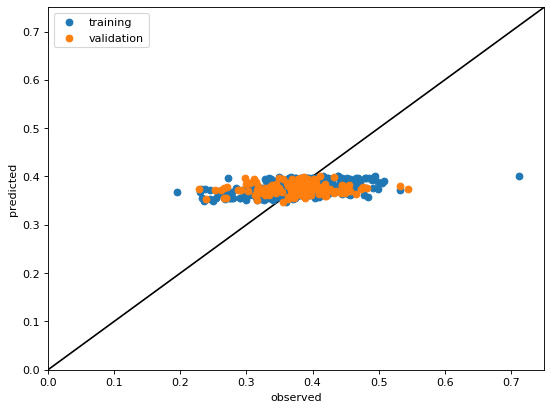
\includegraphics[width=12.0cm, keepaspectratio]{cap3_scatter_random_forest}
\captionof{figure}{Gráfico de dispersão do Random Forest}
\label{ape:cap3_scatter_random_forest}

\section{XGBoost}
\label{sec:xgboost}

O XGBoost (eXtreme Gradient Boosting) é uma implementação do algoritmo Gradient Boosting que é considerado, muitas vezes, melhor que o Gradient Boosting por sua capacidade em reduzir a chance de overfitting. A principal diferença consiste que o XGBoost utiliza uma formalização de modelo mais regularizada, que resulta muitas vezes na redução de overfitting e melhor desempenho.

O nome XGBoost se refere ao objetivo de aumentar o limite de recursos de computação para algoritmos de árvore aprimorada, que é o motivo pelo qual muitas pessoas usam o XGBoost.

O Gradient Boosting é uma técnica de aprendizado de máquina para problemas de regressão e classificação, o algoritmo produz um modelo de previsão na forma de um conjunto de modelos de preditores fracos que são árvores de decisão. A construção do modelo é feita em etapas, como outros métodos de reforço, e os generaliza permitindo a otimização de uma função de perda diferenciável arbitrária. O Gradient Boosting teve origem quando Leo Breiman (ver \citet{Breiman1997}) observou que boosting pode ser interpretado como um algoritmo de otimização em uma função de custo. Sendo que o algoritmo em si foi desenvolvido posteriormente por Jerome H. Friedman (ver \citet{Friedman199902} e \citet{Friedman199903}).

O Gradient Boosting combina preditores fracos em um único preditor forte de maneira iterativa. No exemplo de regressão, na otimização de mínimos quadrados, onde o objetivo é encontrar um modelo $ F $ para prever valores da forma $ \hat{y} = F(x) $ minimizando o erro quadrático médio $ \tfrac{1}{n} \sum_{i} ({\hat{y}}_{i}-y_{i})^{2} $, onde $ i $ é o índice sobre algum conjunto de treinamento de tamanho $ n $ dos valores reais da variável resposta $ y $.

Em cada etapa $ m $, $ 1 \leq m \leq M $ - onde $ M $ é a quantidade de iterações -, do Gradient Boosting, supõe-se que exista algum modelo imperfeito $ F_{m} $ (no início, pode ser usado um modelo muito fraco que prevê apenas a média de $ y $ no conjunto de treinamento). O Gradient Boosting aprimora o $ F_{m} $ construindo um novo modelo que adiciona um estimador $ h $ para fornecer um modelo melhor: $ F_{m + 1}(x) = F_{m}(x) + h(x) $. Para estimar $ h $, o algoritmo começa com a premissa de que um $ h $ perfeito implicaria em

\begin{equation}
F_{m + 1}(x) = F_{m}(x) + h(x) = y
\end{equation}

ou, de forma equivalente,

\begin{equation}
h(x) = y - F_{m}(x)
\end{equation}

Portanto, o Gradient Boosting ajustará $ h $ ao $ y - F_{m}(x) $ e cada $ F_{m + 1} $ tenta corrigir os erros de seu predecessor $ F_{m} $, utilizando a função custo $ L $. Uma generalização dessa idéia para funções de perda que não sejam erros quadráticos e para problemas de classificação, resulta da observação de que os resíduos $ y - F(x) $ para um determinado modelo são os gradientes negativos (em relação à $ F(x) $) da função de perda de erro ao quadrado $ \frac{1}{2} (y - F(x))^{2} $.

Para uma melhor exemplificação, a seguir foi extraído do livro \citet{Hastie2001} o algoritmo do Gradient Boosting e explicado detalhadamente cada passo do mesmo.

\begin{enumerate}
	\item Inicialize $ f_0(x) = \arg \min_{\gamma} \sum^{N}_{i=1} L(y_i, \gamma) $
	\item Para m = 1 até M:
	\begin{enumerate}
    	\item Para $ i = 1,2,...,N $ calcule:
        	\begin{equation}
        	    r_{im} = -\left[\frac{\partial L(y_i, f(x_i))}{\partial f(x_i)}\right]_{f=f_{m-1}} \quad
        	\end{equation}
    	\item Treine uma árvore de regressão sobre a variável resposta resíduo $ r_{im} $ resultando nas regiões $ R_{jm} $, $ j = 1,2,...,J_m $.
    	\item Para $ j = 1,2,...,J_m $ calcule:
    	    \begin{equation}
    	        \gamma_{jm} = \arg \min_{\gamma} \sum_{x_i \in R_{jm}} L(y_i, f_{m-1}(x_i) + \gamma)
    	    \end{equation}
    	\item Atualize $ f_{m}(x) = f_{{m-1}}(x)+ \sum_{j=1}^{J_m} \gamma_{jm} I(x \in R_{jm}) $
	\end{enumerate}
	\item Resultado é $ \hat{f}(x) = f_M(x) $
\end{enumerate}

Sendo que,

\begin{itemize}
	\item Em 1., inicializa-se a primeira iteração ou árvore ($ f_0 $, ou seja, $ m=0 $).
	\item Em 2., o valor M representa o total de iterações (ou árvores).
	\item Em 2.(a), para cada observação i - de um total de N - calcula-se o resíduo dado pelo negativo do gradiente da função perda avaliado em $ f_{m-1} $, por exemplo, no caso de regressão o resultante do gradiente poderia ser $ y_i - f(x_i) $ resultante da função perda $ \frac{1}{2} (y - F(x))^{2} $.
	\item Em 2.(b), treina-se uma árvore de regressão sobre a variável resposta resíduo, sendo que $ J_m $ seria o número total de folhas da referida iteração.
	\item Em 2.(c), calcula-se o argumento que minimiza a função perda para cada folha da referida iteração sobre a predição de $ f_{m-1} $.
	\item Em 2.(d), atualiza-se a função $ f_m(x) $ utilizando-se a função resultante da iteração anterior ($ f_{m-1}(x) $) e o argumento calculado no item anterior ($ \gamma_{jm} $) aplicado apenas aos casos em que o registro pertence à folha em questão ($ x \in R_{jm} $).
	\item O resultado final se dá pela função da última iteração (M).
\end{itemize}

No algoritmo XGBoost, o tamanho da árvore e a magnitude dos pesos são controlados por parâmetros com regularização padrão. Uma infinidade de parâmetros é usada ainda para controlar o tamanho e a forma das árvores. A regularização de tais parâmetros, no entanto, provou ser muito poderosa e fez o algoritmo se tornar muito robusto, sendo que, atualmente, é um dos mais utilizados em competições de aprendizado de máquina.

Neste trabalho, o treinamento do XGBoost foi feito utilizando-se a biblioteca em Python xgboost (\citet{Xgboost}) na linguagem de programação Python.

\section{Resultados do XGBoost}
\label{sec:resultados_xgboost}

O treinamento do modelo XGBoost utilizou-se da metodologia explicada na Seção \ref{sec:randomized_search} e os hiperparâmetros testados foram:

\begin{itemize}
	\item \verb|max_depth|: Profundidade máxima de uma árvore. Aumentar esse valor tornará o modelo mais complexo e mais propenso à overfitting.
	\item \verb|learning_rate|: Define o tamanho da etapa na otimização do algoritmo, usado na atualização dos estimadores servindo para controlar o ajuste a cada etapa.
	\item \verb|colsample_bytree|: Taxa de subamostra de variáveis explicativas ao construir cada árvore. A subamostragem ocorre uma vez para cada árvore construída.
	\item \verb|colsample_bylevel|: Taxa de subamostra de variáveis explicativas para cada nível de profundidade. A subamostragem ocorre uma vez para cada novo nível de profundidade alcançado em uma árvore.
	\item \verb|min_child_weight|: Soma mínima do peso do nó necessária em cada árvore.
	\item \verb|gamma|: Valor mínimo para redução da função perda necessária para fazer uma partição adicional em um nó da árvore. Quanto maior, mais conservador será o algoritmo.
	\item \verb|reg_lambda|: Peso dos termos de regularização L2. Aumentar esse valor tornará o modelo mais conservador.
	\item \verb|n_estimators|: Número de estimadores ou árvores construídas no treinamento.
	\item \verb|eval_metric|: Função a ser usada para medir a qualidade da divisão da árvore (erro quadrático médio, erro absoluto médio, etc.).
\end{itemize}

O número de iterações no Randomized Search a serem realizadas foi de 300 com um método de validação cruzada 5-fold (\citet{Kohavi1995}). Por fim, o modelo final após a otimização do Randomized Search possui os hiperparâmetros apresentados na tabela abaixo.

\begin{table}[h]
\centering
\caption{Hiperparâmetros finais do Xgboost}
\label{tab:cap3_parametros_xgboost}
\begin{tabular}{cc}
Hiperparâmetro & Valor \\
\hline
\verb|max_depth| & 12 \\
\verb|learning_rate| & 0.1 \\
\verb|colsample_bytree| & 0.4 \\
\verb|colsample_bylevel| & 0.7 \\
\verb|min_child_weight| & 7.0 \\
\verb|gamma| & 0 \\
\verb|reg_lambda| & 100.0 \\
\verb|n_estimators| & 50 \\
\verb|eval_metric| & rmse \\
\hline
\end{tabular}
\end{table}
\FloatBarrier

O modelo XGBoost não é de fácil interpretabilidade, apesar de ser possível ver e analisar a estrutura de cada uma das árvores separadamente que compõem o mesmo, não é direta a interpretação de como foi feita a predição dos valores por tal algoritmo. Assim, para interpretar como cada variável afeta o modelo e avaliar a importância de cada uma delas utilizamos o método de Shapley Values (descrito na Seção \ref{sec:shapley_value}) e o gráfico resultante se encontra abaixo.

\graphicspath{ {./figuras/model_performance/} }
\begin{center}
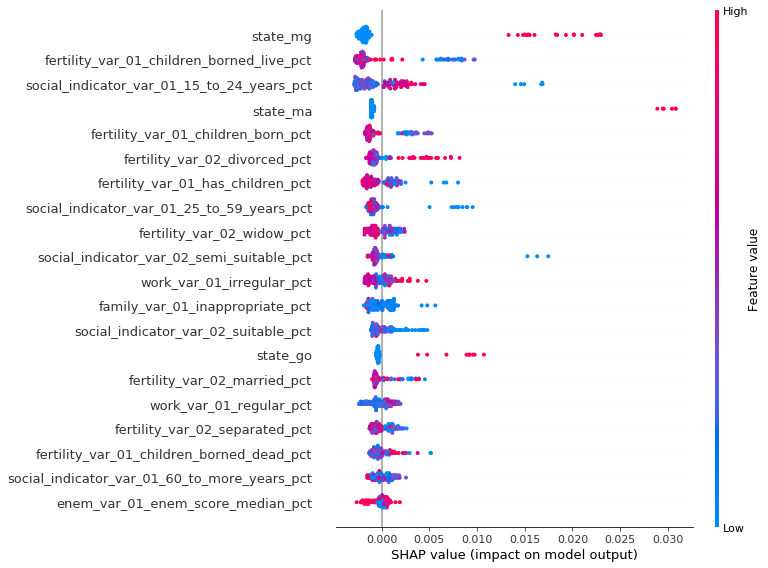
\includegraphics[width=14.0cm, keepaspectratio]{cap3_shap_xgboost}
\captionof{figure}{Shapley value do Xgboost}
\label{ape:cap3_shap_xgboost}
\end{center}

No gráfico, as variáveis apresentadas à esquerda estão ordenadas de forma decrescente em nível de importância no modelo, no eixo das ordenadas se apresentam os valores de Shapley Values - que pode ser lido como a influência no valor de predição do modelo, tanto positivo quanto negativo -, e as cores como o valor da variável explicativa propriamente dita, sendo vermelho o maior valor possível e azul o menor valor possível para a variável em questão. Então, no caso da variável \verb|state_mg| - que se trata do estado de origem do município avaliado -, a interpretação se dá na forma de que quanto maior o valor de tal variável (neste caso um, por se tratar de uma variável binária), mais positiva será a influência sobre a predição de polaridade negativa no relatório do município em questão.

Assim como a regressão linear, o desempenho do modelo foi avaliado utilizando-se as medidas RMSE e bandas de acerto. Na tabela abaixo apresenta-se o RMSE sobre a base de treinamento ("Treino"), sobre a base de validação ("Validação"), sobre a base de validação utilizando-se um modelo aleatório ("Validação (modelo aleatório)") e sobre a base de validação utilizando-se um modelo nulo ("Validação (modelo nulo)"). O modelo aleatório apresenta um número aleatório que esteja entre o mínimo e o máximo observado na validação, foi criado apenas para critério de comparação com o modelo XGBoost, assim como o modelo nulo, sendo que o modelo nulo é a média da variável resposta na base de treinamento. Nota-se um erro estritamente superior do modelo aleatório sobre o erro do XGBoost.

\begin{table}[h]
\centering
\caption{RMSE resultante do Xgboost}
\label{tab:cap3_rmse_xgboost}
\begin{tabular}{cc}
Base & Estatística \\
\hline
Treino & 0.0448 \\
Validação & 0.0521 \\
Validação (modelo aleatório) & 0.1814 \\
Validação (modelo nulo) & 0.0525 \\
\hline
\end{tabular}
\end{table}
\FloatBarrier

Na tabela abaixo apresenta-se a banda de acerto sobre a base de treinamento ("Treino"), sobre a base de validação ("Validação"), sobre a base de validação utilizando-se um modelo aleatório ("Validação (modelo aleatório)") e sobre a base de validação utilizando-se um modelo nulo ("Validação (modelo nulo)"). Nota-se que o XGBoost teve a maior concentração em "Bem Estimado" com mais de 70\% na validação e quase 80\% no treino.

\begin{table}[h]
\centering
\caption{Banda de acerto do Xgboost}
\label{tab:cap3_band_xgboost}
\begin{tabular}{cccc}
Base & Subestimado & Bem Estimado & Superestimado \\
\hline
Treino & 0.0929 & 0.7976 & 0.1095 \\
Validação & 0.1071 & 0.7215 & 0.1714 \\
Validação (modelo aleatório) & 0.4429 & 0.1642 & 0.3929 \\
Validação (modelo nulo) & 0.1214 & 0.7143 & 0.1643 \\
\hline
\end{tabular}
\end{table}

No gráfico abaixo nota-se, apesar de suave, uma relação de linearidade entre os valores preditos (eixo das ordenadas) e os valores observados (eixo das abscissas) em ambas bases de dados (treino e validação).

\graphicspath{ {./figuras/model_performance/} }
\begin{center}
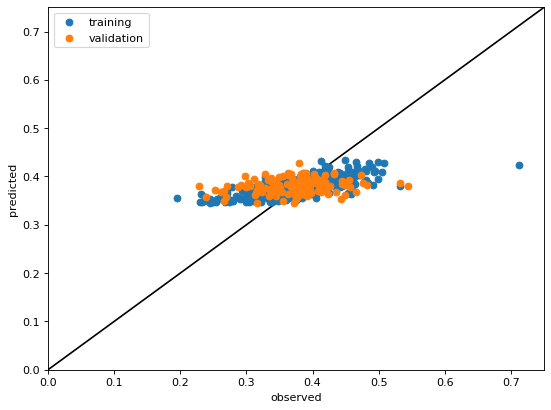
\includegraphics[width=12.0cm, keepaspectratio]{cap3_scatter_xgboost}
\captionof{figure}{Gráfico de dispersão do Xgboost}
\label{ape:cap3_scatter_xgboost}
\end{center}

%% ------------------------------------------------------------------------- %%